%%%%%%%%%%%%%%%%%%%%%%%%%%%%%%%%%%%%%%%%
% datoteka diploma-vzorec.tex
%
% vzorčna datoteka za pisanje diplomskega dela v formatu LaTeX
% na UL Fakulteti za računalništvo in informatiko
%
% vkup spravil Gašper Fijavž, december 2010
% 
%
%
% verzija 12. februar 2014 (besedilo teme, seznam kratic, popravki Gašper Fijavž)
% verzija 10. marec 2014 (redakcijski popravki Zoran Bosnić)
% verzija 11. marec 2014 (redakcijski popravki Gašper Fijavž)
% verzija 15. april 2014 (pdf/a 1b compliance, not really - just claiming, Damjan Cvetan, Gašper Fijavž)
% verzija 23. april 2014 (privzeto cc licenca)
% verzija 16. september 2014 (odmiki strain od roba)
% verzija 28. oktober 2014 (odstranil vpisno številko)
% verija 5. februar 2015 (Literatura v kazalu, online literatura)
% verzija 25. september 2015 (angl. naslov v izjavi o avtorstvu)
% verzija 26. februar 2016 (UL izjava o avtorstvu)
% verzija 16. april 2016 (odstranjena izjava o avtorstvu)
% verzija 5. junij 2016 (Franc Solina dodal vrstice, ki jih je označil s svojim imenom)


\documentclass[a4paper, 12pt]{book}
%\documentclass[a4paper, 12pt, draft]{book}  Nalogo preverite tudi z opcijo draft, ki vam bo pokazala, katere vrstice so predolge!



\usepackage[utf8x]{inputenc}   % omogoča uporabo slovenskih črk kodiranih v formatu UTF-8
\usepackage[slovene,english]{babel}    % naloži, med drugim, slovenske delilne vzorce
\usepackage[pdftex]{graphicx}  % omogoča vlaganje slik različnih formatov
\usepackage{fancyhdr}          % poskrbi, na primer, za glave stranif
\usepackage{amssymb}           % dodatni simboli
\usepackage{amsmath}           % eqref, npr.
%\usepackage{hyperxmp}
\usepackage[hyphens]{url}  % dodal Solina
\usepackage{comment}       % dodal Solina

\usepackage[pdftex, colorlinks=true,
						citecolor=black, filecolor=black, 
						linkcolor=black, urlcolor=black,
						pagebackref=false, 
						pdfproducer={LaTeX}, pdfcreator={LaTeX}, hidelinks]{hyperref}

\usepackage{color}       % dodal Solina
\usepackage{soul}       % dodal Solina

%%%%%%%%%%%%%%%%%%%%%%%%%%%%%%%%%%%%%%%%
%	DIPLOMA INFO
%%%%%%%%%%%%%%%%%%%%%%%%%%%%%%%%%%%%%%%%
\newcommand{\ttitle}{Elektronsko naročanje v restavraciji}
\newcommand{\ttitleEn}{Diploma thesis sample}
\newcommand{\tsubject}{\ttitle}
\newcommand{\tsubjectEn}{\ttitleEn}
\newcommand{\tauthor}{Luka Horvat}
\newcommand{\tkeywords}{Slovenija, naročanje, neuspešni projekti, rešitev, spletna aplikacija}
\newcommand{\tkeywordsEn}{computer, computer, computer}


%%%%%%%%%%%%%%%%%%%%%%%%%%%%%%%%%%%%%%%%
%	HYPERREF SETUP
%%%%%%%%%%%%%%%%%%%%%%%%%%%%%%%%%%%%%%%%
\hypersetup{pdftitle={\ttitle}}
\hypersetup{pdfsubject=\ttitleEn}
\hypersetup{pdfauthor={\tauthor, matjaz.kralj@fri.uni-lj.si}}
\hypersetup{pdfkeywords=\tkeywordsEn}


 


%%%%%%%%%%%%%%%%%%%%%%%%%%%%%%%%%%%%%%%%
% postavitev strani
%%%%%%%%%%%%%%%%%%%%%%%%%%%%%%%%%%%%%%%%  

\addtolength{\marginparwidth}{-20pt} % robovi za tisk
\addtolength{\oddsidemargin}{40pt}
\addtolength{\evensidemargin}{-40pt}

\renewcommand{\baselinestretch}{1.3} % ustrezen razmik med vrsticami
\setlength{\headheight}{15pt}        % potreben prostor na vrhu
\renewcommand{\chaptermark}[1]%
{\markboth{\MakeUppercase{\thechapter.\ #1}}{}} \renewcommand{\sectionmark}[1]%
{\markright{\MakeUppercase{\thesection.\ #1}}} \renewcommand{\headrulewidth}{0.5pt} \renewcommand{\footrulewidth}{0pt}
\fancyhf{}
\fancyhead[LE,RO]{\sl \thepage} 
%\fancyhead[LO]{\sl \rightmark} \fancyhead[RE]{\sl \leftmark}
\fancyhead[RE]{\sc \tauthor}              % dodal Solina
\fancyhead[LO]{\sc Diplomska naloga}     % dodal Solina


\newcommand{\BibTeX}{{\sc Bib}\TeX}

%%%%%%%%%%%%%%%%%%%%%%%%%%%%%%%%%%%%%%%%
% naslovi
%%%%%%%%%%%%%%%%%%%%%%%%%%%%%%%%%%%%%%%%  


\newcommand{\autfont}{\Large}
\newcommand{\titfont}{\LARGE\bf}
\newcommand{\clearemptydoublepage}{\newpage{\pagestyle{empty}\cleardoublepage}}
\setcounter{tocdepth}{2}	      % globina kazala

%%%%%%%%%%%%%%%%%%%%%%%%%%%%%%%%%%%%%%%%
% konstrukti
%%%%%%%%%%%%%%%%%%%%%%%%%%%%%%%%%%%%%%%%  
\newtheorem{izrek}{Izrek}[chapter]
\newtheorem{trditev}{Trditev}[izrek]
\newenvironment{dokaz}{\emph{Dokaz.}\ }{\hspace{\fill}{$\Box$}}

%%%%%%%%%%%%%%%%%%%%%%%%%%%%%%%%%%%%%%%%%%%%%%%%%%%%%%%%%%%%%%%%%%%%%%%%%%%%%%%
%% PDF-A
%%%%%%%%%%%%%%%%%%%%%%%%%%%%%%%%%%%%%%%%%%%%%%%%%%%%%%%%%%%%%%%%%%%%%%%%%%%%%%%


%%%%%%%%%%%%%%%%%%%%%%%%%%%%%%%%%%%%%%%% 
% define medatata
%%%%%%%%%%%%%%%%%%%%%%%%%%%%%%%%%%%%%%%% 
\def\Title{\ttitle}
\def\Author{\tauthor, lh8069@fri.uni-lj.si}
\def\Subject{\ttitleEn}
\def\Keywords{\tkeywordsEn}

%%%%%%%%%%%%%%%%%%%%%%%%%%%%%%%%%%%%%%%% 
% \convertDate converts D:20080419103507+02'00' to 2008-04-19T10:35:07+02:00
%%%%%%%%%%%%%%%%%%%%%%%%%%%%%%%%%%%%%%%% 
\def\convertDate{%
    \getYear
}

{\catcode`\D=12
 \gdef\getYear D:#1#2#3#4{\edef\xYear{#1#2#3#4}\getMonth}
}
\def\getMonth#1#2{\edef\xMonth{#1#2}\getDay}
\def\getDay#1#2{\edef\xDay{#1#2}\getHour}
\def\getHour#1#2{\edef\xHour{#1#2}\getMin}
\def\getMin#1#2{\edef\xMin{#1#2}\getSec}
\def\getSec#1#2{\edef\xSec{#1#2}\getTZh}
\def\getTZh +#1#2{\edef\xTZh{#1#2}\getTZm}
\def\getTZm '#1#2'{%
    \edef\xTZm{#1#2}%
    \edef\convDate{\xYear-\xMonth-\xDay T\xHour:\xMin:\xSec+\xTZh:\xTZm}%
}

\expandafter\convertDate\pdfcreationdate 

%%%%%%%%%%%%%%%%%%%%%%%%%%%%%%%%%%%%%%%%
% get pdftex version string
%%%%%%%%%%%%%%%%%%%%%%%%%%%%%%%%%%%%%%%% 
\newcount\countA
\countA=\pdftexversion
\advance \countA by -100
\def\pdftexVersionStr{pdfTeX-1.\the\countA.\pdftexrevision}


%%%%%%%%%%%%%%%%%%%%%%%%%%%%%%%%%%%%%%%%
% XMP data
%%%%%%%%%%%%%%%%%%%%%%%%%%%%%%%%%%%%%%%%  
\usepackage{xmpincl}
\includexmp{pdfa-1b}

%%%%%%%%%%%%%%%%%%%%%%%%%%%%%%%%%%%%%%%%
% pdfInfo
%%%%%%%%%%%%%%%%%%%%%%%%%%%%%%%%%%%%%%%%  
\pdfinfo{%
    /Title    (\ttitle)
    /Author   (\tauthor, damjan@cvetan.si)
    /Subject  (\ttitleEn)
    /Keywords (\tkeywordsEn)
    /ModDate  (\pdfcreationdate)
    /Trapped  /False
}


%%%%%%%%%%%%%%%%%%%%%%%%%%%%%%%%%%%%%%%%%%%%%%%%%%%%%%%%%%%%%%%%%%%%%%%%%%%%%%%
%%%%%%%%%%%%%%%%%%%%%%%%%%%%%%%%%%%%%%%%%%%%%%%%%%%%%%%%%%%%%%%%%%%%%%%%%%%%%%%

\begin{document}
\selectlanguage{slovene}
\frontmatter
\setcounter{page}{1} %
\renewcommand{\thepage}{}       % preprecimo težave s številkami strani v kazalu
\newcommand{\sn}[1]{"`#1"'}                    % dodal Solina (slovenski narekovaji)

%%%%%%%%%%%%%%%%%%%%%%%%%%%%%%%%%%%%%%%%
%naslovnica
 \thispagestyle{empty}%
   \begin{center}
    {\large\sc Univerza v Ljubljani\\%
      Fakulteta za računalništvo in informatiko}%
    \vskip 10em%
    {\autfont \tauthor\par}%
    {\titfont \ttitle \par}%
    {\vskip 3em \textsc{DIPLOMSKO DELO\\[5mm]         % dodal Solina za ostale študijske programe
%    VISOKOŠOLSKI STROKOVNI ŠTUDIJSKI PROGRAM\\ PRVE STOPNJE\\ RAČUNALNIŠTVO IN INFORMATIKA}\par}%
    VISOKOŠOLSKI ŠTUDIJSKI PROGRAM \\ PRVE STOPNJE\\ RAČUNALNIŠTVO IN INFORMATIKA}\par}%
%    INTERDISCIPLINARNI UNIVERZITETNI\\ ŠTUDIJSKI PROGRAM PRVE STOPNJE\\ RAČUNALNIŠTVO IN MATEMATIKA}\par}%
%    INTERDISCIPLINARNI UNIVERZITETNI\\ ŠTUDIJSKI PROGRAM PRVE STOPNJE\\ UPRAVNA INFORMATIKA}\par}%
%    INTERDISCIPLINARNI UNIVERZITETNI\\ ŠTUDIJSKI PROGRAM PRVE STOPNJE\\ MULTIMEDIJA}\par}%
    \vfill\null%
    {\large \textsc{Mentorica}: doc. dr. Mira Trebar\par}%
   {\large \textsc{Somentor}: as. dr. David Jelenc \par}%
    {\vskip 2em \large Ljubljana, 2021 \par}%
\end{center}
% prazna stran
%\clearemptydoublepage      % dodal Solina (izjava o licencah itd. se izpiše na hrbtni strani naslovnice)

%%%%%%%%%%%%%%%%%%%%%%%%%%%%%%%%%%%%%%%%
%copyright stran
\thispagestyle{empty}
\vspace*{8cm}

\noindent
{\sc Copyright}. 
Rezultati diplomske naloge so intelektualna lastnina avtorja in Fakultete za računalništvo in informatiko Univerze v Ljubljani.
Za objavo in koriščenje rezultatov diplomske naloge je potrebno pisno privoljenje avtorja, Fakultete za računalništvo in informatiko ter mentorja.

\begin{center}
\mbox{}\vfill
\emph{Besedilo je oblikovano z urejevalnikom besedil \LaTeX.}
\end{center}
% prazna stran
\clearemptydoublepage

%%%%%%%%%%%%%%%%%%%%%%%%%%%%%%%%%%%%%%%%
% stran 3 med uvodnimi listi
\thispagestyle{empty}
\vspace*{4cm}

\noindent
Fakulteta za računalništvo in informatiko izdaja naslednjo nalogo:
\medskip
\begin{tabbing}
\hspace{32mm}\= \hspace{6cm} \= \kill




Tematika naloge: Elektronsko naročanje v restavracij
\end{tabbing}
Besedilo teme diplomskega dela študent prepiše iz študijskega informacijskega sistema, kamor ga je vnesel mentor. V nekaj stavkih bo opisal, kaj pričakuje od kandidatovega diplomskega dela. Kaj so cilji, kakšne metode uporabiti, morda bo zapisal tudi ključno literaturo.
\vspace{15mm}






\vspace{2cm}

% prazna stran
\clearemptydoublepage

% zahvala
\thispagestyle{empty}\mbox{}\vfill\null\it%
\noindent
Na tem mestu zapišite, komu se zahvaljujete za izdelavo diplomske naloge. Pazite, da ne boste koga pozabili. Utegnil vam bo zameriti. Temu se da izogniti tako, da celotno zahvalo izpustite.
\rm\normalfont

% prazna stran
\clearemptydoublepage

%%%%%%%%%%%%%%%%%%%%%%%%%%%%%%%%%%%%%%%%
% posvetilo, če sama zahvala ne zadošča :-)
%\thispagestyle{empty}\mbox{}{\vskip0.20\textheight}\mbox{}\hfill\begin{minipage}{0.55\textwidth}%
%Svoji dragi Alenčici.
%\normalfont\end{minipage}

% prazna stran
\clearemptydoublepage


%%%%%%%%%%%%%%%%%%%%%%%%%%%%%%%%%%%%%%%%
% kazalo
\pagestyle{empty}
\def\thepage{}% preprecimo tezave s stevilkami strani v kazalu
\tableofcontents{}

% prazna stran
\clearemptydoublepage

%%%%%%%%%%%%%%%%%%%%%%%%%%%%%%%%%%%%%%%%
% seznam kratic

\chapter*{Seznam uporabljenih kratic}  % spremenil Solina, da predolge vrstice ne gredo preko desnega roba

\begin{comment}
\begin{tabular}{l|l|l}
  {\bf kratica} & {\bf angleško} & {\bf slovensko} \\ \hline
  % after \\: \hline or \cline{col1-col2} \cline{col3-col4} ...
  {\bf SPA} & single page application & aplikacija na eni strani \\
  {\bf SQL} & structured query language & strukturirani povpraševalni jezik za delo s podatkovnimi bazami  \\
  {\bf SVM} & support vector machine & metoda podpornih vektorjev \\
  {\bf SVM}   & support vector machine              & metoda podpornih vektorjev \\
  \dots & \dots & \dots \\
\end{tabular}
\end{comment}

\noindent\begin{tabular}{p{0.1\textwidth}|p{.4\textwidth}|p{.4\textwidth}}    % po potrebi razširi prvo kolono tabele na račun drugih dveh!
  {\bf kratica} & {\bf angleško}                             & {\bf slovensko} \\ \hline
  {\bf SPA}      & single page application               &  aplikacija na eni strani \\
  {\bf SQL} & structured query language & strukturirani povpraševalni jezik za delo s podatkovnimi bazami  \\
  {\bf CLI}   & command-line interface              & znakovni uporabniški vmesnik \\
  {\bf REST}   & representational state transfer              & aktualni prenos stanja \\
  {\bf URI}   &  uniform resource identifier              & enotni identifikator vira \\
  {\bf SPA}   &  single-page application              & aplikacija na eni strani \\
%  \dots & \dots & \dots \\
\end{tabular}


% prazna stran
\clearemptydoublepage

%%%%%%%%%%%%%%%%%%%%%%%%%%%%%%%%%%%%%%%%
% povzetek
\addcontentsline{toc}{chapter}{Povzetek}
\chapter*{Povzetek}

\noindent\textbf{Naslov:} \ttitle
\bigskip

\noindent\textbf{Avtor:} \tauthor
\bigskip

%\noindent\textbf{Povzetek:} 
\noindent 
Pride na koncu.

\noindent\textbf{Ključne besede:} \tkeywords.
% prazna stran
\clearemptydoublepage

%%%%%%%%%%%%%%%%%%%%%%%%%%%%%%%%%%%%%%%%
% abstract
\selectlanguage{english}
\addcontentsline{toc}{chapter}{Abstract}
\chapter*{Abstract}

\noindent\textbf{Title:} \ttitleEn
\bigskip

\noindent\textbf{Author:} \tauthor
\bigskip

%\noindent\textbf{Abstract:} 
\noindent This sample document presents an approach to typesetting your BSc thesis using \LaTeX. 
A proper abstract should contain around 100 words which makes this one way too short.
\bigskip

\noindent\textbf{Keywords:} \tkeywordsEn.
\selectlanguage{slovene}
% prazna stran
\clearemptydoublepage

%%%%%%%%%%%%%%%%%%%%%%%%%%%%%%%%%%%%%%%%
\mainmatter
\setcounter{page}{1}
\pagestyle{fancy}

\chapter{Uvod}
Slovenija velja za državo z veliko število restavracij, vendar le malo iz med njih uporablja napredne sisteme naročanja kot npr. ena izmed večjih verig s hitro prehrano, McDonalds. V Sloveniji je bilo nekaj projektov s podobnimi idejami, vendar z napačnimi cilji zaradi katerih so bili neuspešni. Eden izmed razlogov da jim ni uspelo je bilo sabotiranje sistemov s strani natakarjev, saj so misli da bo tehnologija zamenjala njegove službe. V zavedanju teh problematik smo se odločil narediti diplomski nalogo na to temo. 

Zamislili smo si sistem za oddajanje naročil v restavracijah, ki ne bi bil namenjen zamenjavi ljudi v strežbi, temveč kot pregledovalnik (angl. Menu) oziroma naročanju hrane in pijače. Aplikacija za stranke bi bila na tablicah, ki bi bile locirane na vsaki mizi restavracije. Stranka bi bila tista, ki bi se odločila ali želi pri naročanju uporabiti stik z osebo v strežbi ali bi naročila z uporabo aplikacije na tablici. Natakar bi tako imel več časa, katerega bi lahko posvetil pripravi pijače, kvaliteti postrežbe in ostalih dolžnosti. Tudi stranke, katere sedaj veljajo za bolj zahtevne in neučakane na vseh področij, bi bile hitreje in bolj kvalitetno postrežene. Tako bi imeli poleg restavracij z hitro prehrano tudi restavracije s hitro postrežbo. 

Aplikacija podpira tri uporabniške vloge, in sicer gost, natakar in kuhar. 

\chapter{Razvoj in struktura aplikacije}

Razvoj aplikacije je potekal v treh delih in sicer analiza problematike oziroma izdelava diagrama primerov uporabe, zamisel strukture in implementacija.

Iz analize zahtev smo za lažji pregled nad vsemi funkcionalnostmi izdelali diagram primerov uporabe, ki ga prikazuje slika~\ref{FunkVloge}.

\begin{figure}[!htb]
\begin{center}
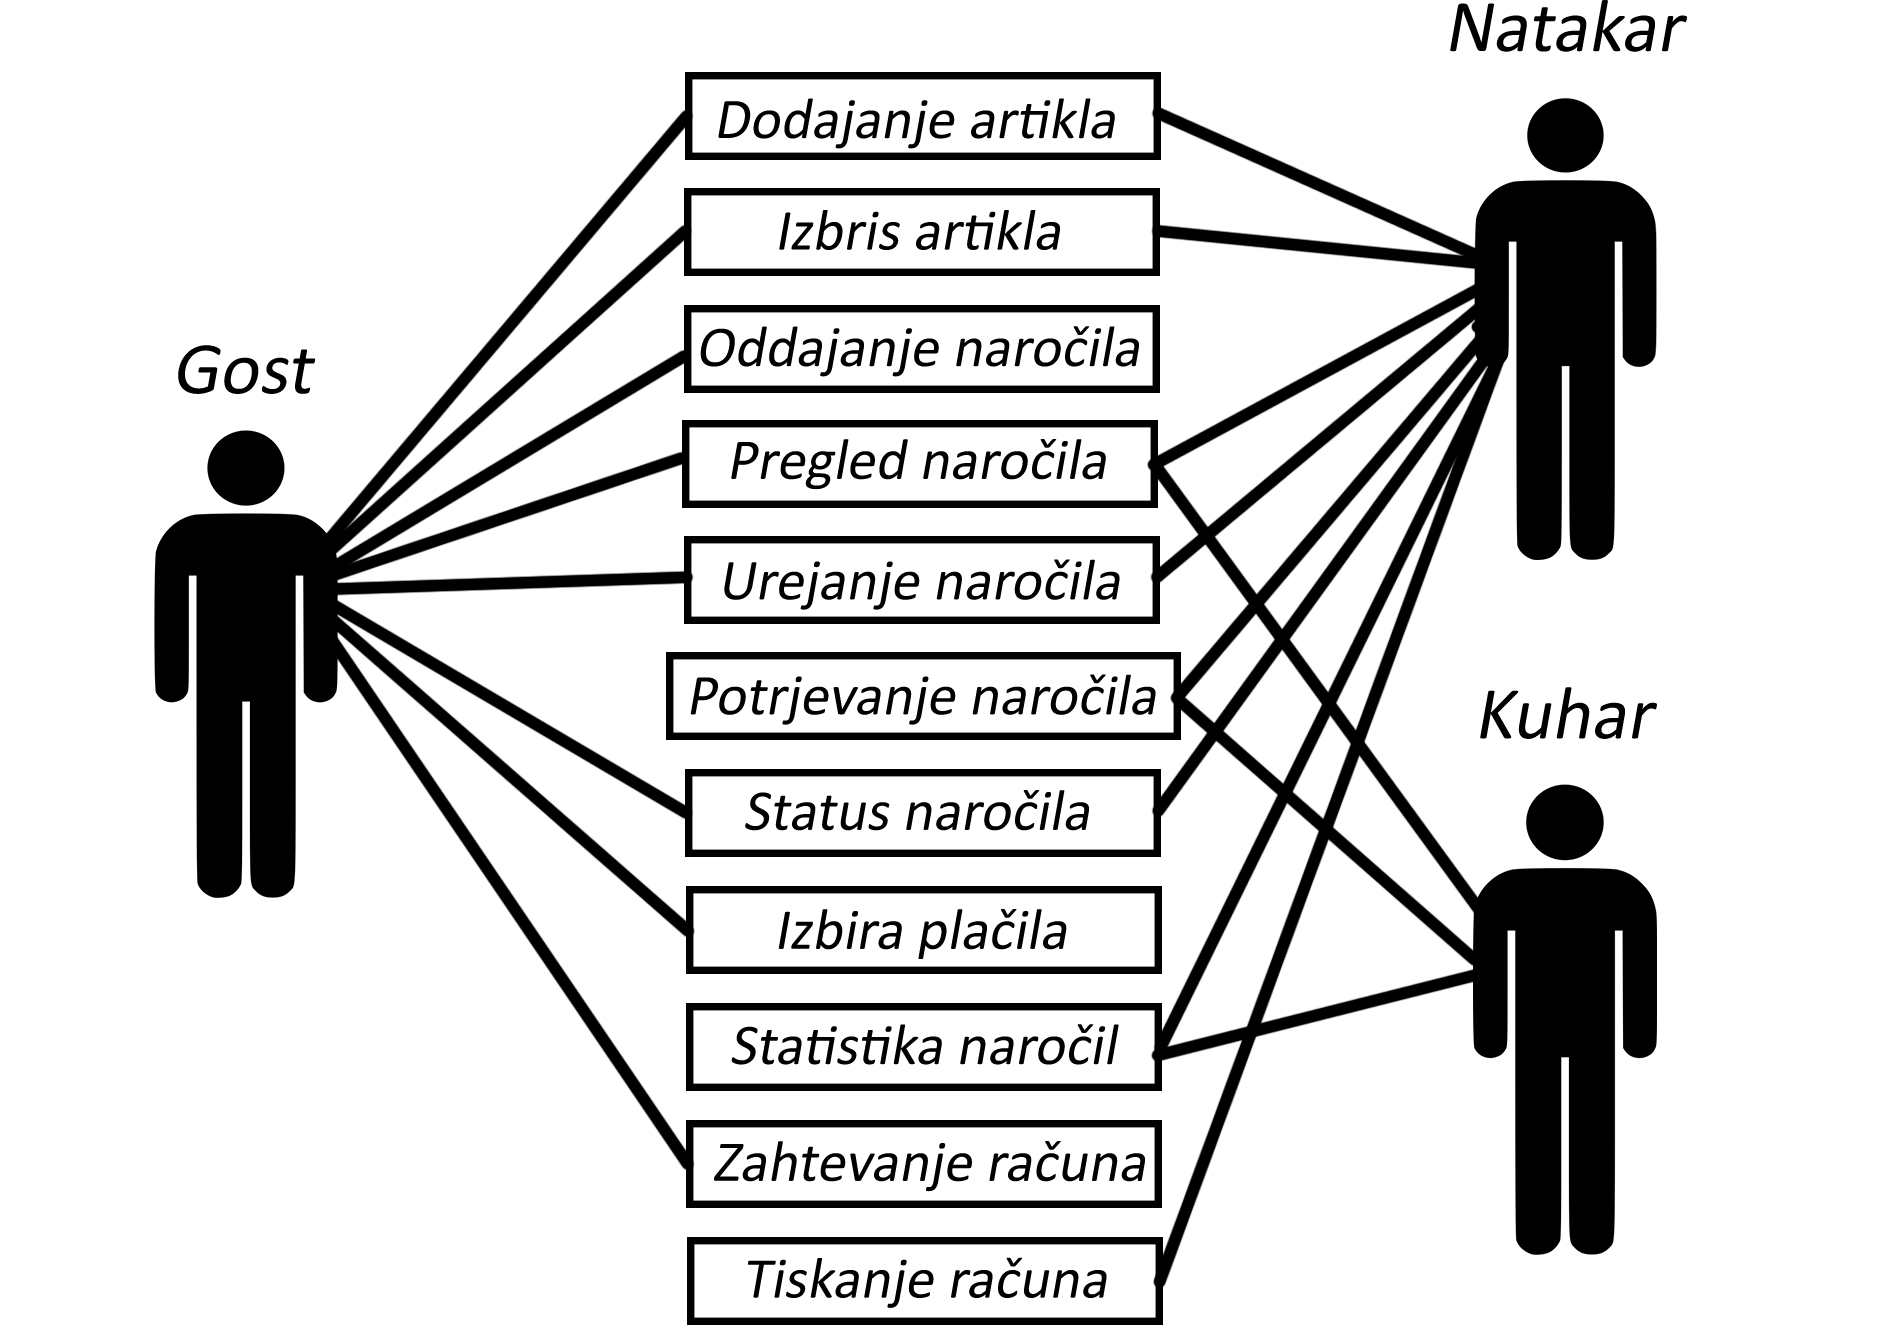
\includegraphics[width=12cm]{Skica2.png}
\end{center}
\caption{Diagram primerov uporabe spretnega naročanja}
\label{FunkVloge}
\end{figure}
Aplikacija oziroma odjemalec ima tri uporabniške poglede, ki so gost, natakar in kuhar. Restavracija ima lahko več miz, vendar za eno mizo je lahko hkrati odprto eno naročilo. To pomeni, da morajo za mizo naročati skupaj. Gost lahko odda, spremeni ali zaključi naročilo. 
Natakar lahko sprejme, zavrne, uredi ali zaključi naročilo.  V restavraciji je lahko več natakarjev, ki streže istočasno.  Kuhar lahko sprejeme, zavrne ali sporoči, da jed za neko naročilo že pripravljena. Restavracija ima lahko več kuharjev, vendar samo en kuhar hkrati lahko uporablja aplikacijo. Omejitev je v podatkovnem modelu.


Uporabili smo strukturo novodobnih aplikacij katero sestavljajo podatkovna baza, strežnik in odjemalca. Gre za koncept, ki ga je moč prilagajati predvsem z uporabniškega vidika. Slika~\ref{StrukApk} prikazuje strukturo aplikacije.

\begin{figure}[!htb]
\centering
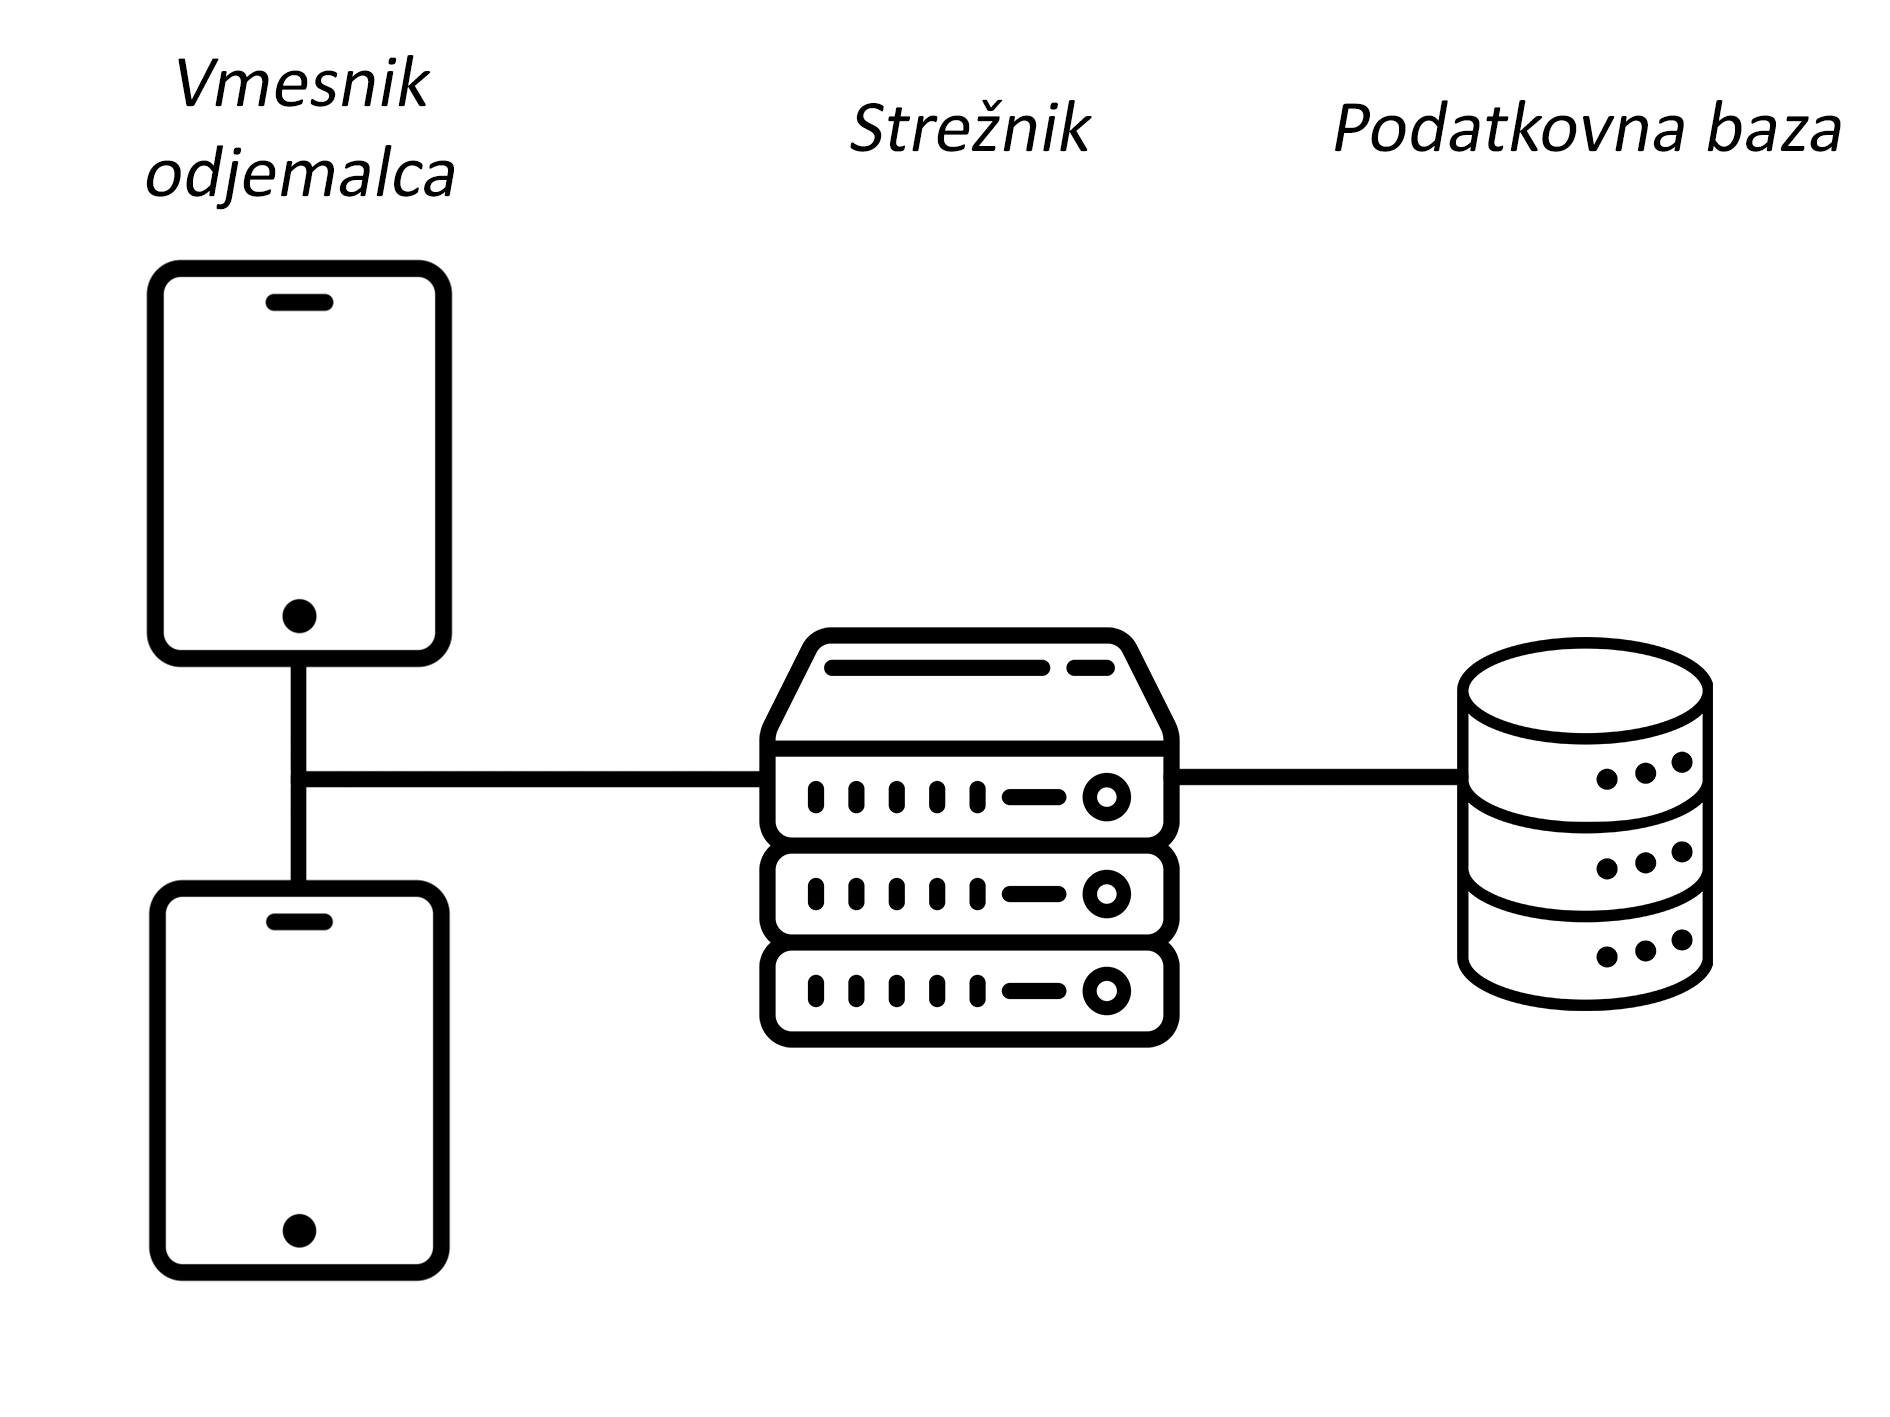
\includegraphics[width=11cm]{Skica1.png}
\caption{Visokonivojska arhitektura}
\label{StrukApk}
\end{figure}

Podatkovna baza je namenjena shranjevanju vseh podatkov, da se ne izgubijo ter se razlikujejo za vsako restavracijo. 
Strežnik implementira RESTful vmesnik, ki odjemalcu servira podatke iz podatkovne baze. Odjemalec sta v našem primeru dve aplikaciji implementirani s pomočjo spletnih tehnologij.


 

\section{Podatkovna baza}
Na podlagi izdelanega diagrama zahtev oziroma fukcij smo izdelali logičen podatkovni model (slika~\ref{Database_physical}), katerega smo kasneje realizirali s pomočjo SUPB MySQL. Podatkovna baza je sestavljena je iz šestih tabel, ki so: \textit{ProductType, Product, ProductOrder, Order, User, Table}. 

\begin{figure}[!htb]
\begin{center}
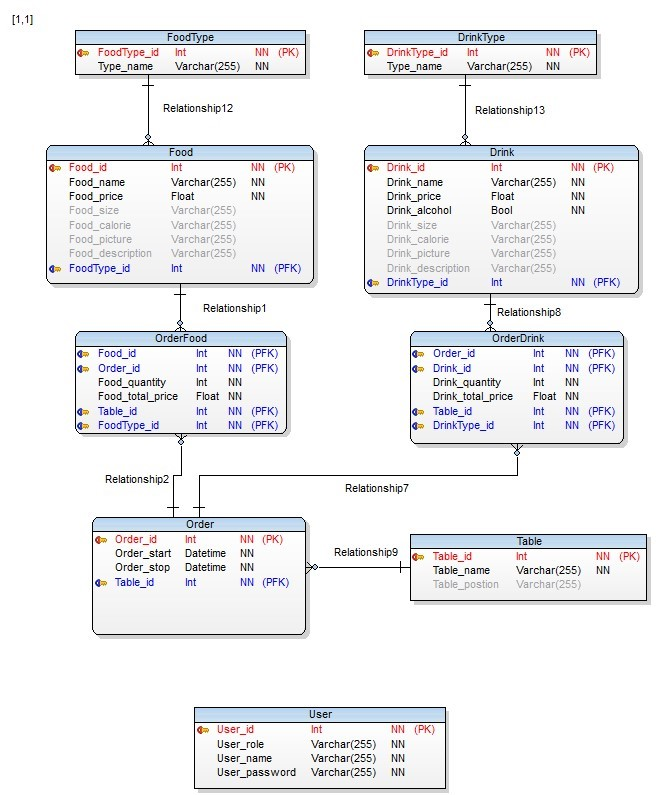
\includegraphics[width=0.85\textwidth]{Database_physical}
\end{center}
\caption{Logični podatkovni model}
\label{Database_physical}
\end{figure}

\textit{ProductType} tabela je namenjana zapisom vrsti jedi t.i. predjedi, glavne jedi, sokovi, piva,… Sestavljena je iz atributov ID, Name in Type. Atribut Type je namenjen razlikovanju hrane in pijače. Uporabljen je za razločevanje artiklov v naročilu, saj kuhar ne potrebuje pregleda nad naročili, ki vsebujejo samo pijače. 

\textit{Product} tabela je namenjena opisu hrane in pijače ter je sestavljena iz atributov: ID, Name, Price, Size, Calorie, Picture in Description.  V atribut Picture se zapiše ime slike, ki se prikaže v aplikaciji. Vse slike smo shranjevali v datotečnem sistemu spletnega strežnika.

\textit{ProductOrder} tabela je namenjena količini in končni ceni vsake hrane in pijače v naročilu. Sestavljena je iz atributov: TotalPrice in Quantity. Zapis ne more obstajati če nima definiranega naročila. Tabela je nastala zaradi razmerja M:N t.i. mnogo-proti-mnogo med tabelo Product in Order.

\textit{Order} tabela je namenjena zapisovanju naročila in njegovih podrobnosti. Sestavljena je iz atributov: ID, Start, End, OrderStatus, CookStatus, Payment. Vsebuje tudi tuji ključ ID od table Table, ki določa, na katero mizo je vezano naročilo. Atributa OrderStatus in CookStatus sta nemanjena sporočanju statusa naročila med vlogami. Uporabil sem ENUM za vrsto parametra, saj gre za vrednosti, ki se ne spreminjajo.

\textit{Table} tabela je namenjena shranjevanju miz v restavracijah. Sestavljajo jo atributi: ID, Name in Position, v katerega se lahko bolj podrobno opiše lokacijo mize.

\textit{User} tabela je namenjena predvsem aplikativnem delu za natakarje in kuharje. Sestavljna je iz atributov: ID, Role, Name in Password. 

Strukturo podatkovne baze smo naredili s pomočjo programa Toad DataModler. To je orodje za izdelavo visokokakovostnih podatkovnih modelov \cite{Toad_Data_Modeler}. Omogoča izdelavo logičnih in fizičnih podatkovnih modelov, kar pripomore k lažjem razumevanju in razvijanju podatkovne baze. Njegova najboljša funkcionalnost je, da lahko generiramo SQL kodo v različne podatkovne sisteme kot npr. MySQL, Ingres, Microsoft Azurem, Microsoft Access, Mircrosoft SQL Server,... 

Podatkovni model smo implementirali na fizičnem nivoju v SUPB MySQL. To je eden od odprtokodnih sistemov za upravljanje s podatkovni bazami, ki za delo s podatki uporablja jezik SQL \cite{MySQL}. Napisan je v programskem jeziku C in C++ in deluje v vseh modernih sistemih npr. Windows, Linux, OS X,… Prva verzija je bil razvita leta 1995 s strani Michael Widenius in David Axmark. Kratica My izhaja iz imena prve hčerke očeta Michaela.  


\section{Strežnik}
Strežnik v naši aplikaciji predstavlja vmesnik med podatkovno bazo in odjemalcem. Ko smo izdelali podatkovno bazo smo začeli z izdelavo strežniškega dela. Najbolj pomembno nam je bilo, da je sistem zanesljiv, saj brez njega odjemalec ne more delovati. Izbrali smo REST arhitekturo zaradi načel, ki so opisana spodaj \cite{RESTAPI}. Sama arhitektura omogoča, da odjemalec s pomočjo zahtev pridobiva podatke od strežnika, kateri jih s pomočjo URI povezav oglašuje na relativnih povezavah.  Strežnik smo napisali v programskem jeziku Python ter s pomočjo knjižnic Flask, MySQL, SocketIO in CORS, kateri nameni so bolj podrobno opisani spodaj. Načela arhitekure REST so sledeča:

1.)\textit{ Odjemalec-strežnik (ang. Client-server)} zahteva ločitev odjemalca od strežnika kar onemogoča odjemalcu direktno povezljivost s podatkovno bazo in s tem poenostavi razširljivost uporabniškega dela. Strežnik ne zanima uporabniški vmesnik ali podatki, tako da je bolj enostaven in prilagodljiv za uporabo. Tako se lahko uporabniški kot strežniški del razvija ali zamenjuje neodvisno. V naši aplikaciji imamo kar dva odjemalca (gost in natakar/kuhar), kar pa za strežnik ne predstavlja nobenih omejitev razen na strani podatkovne baze, ki omejuje število hkratnih poizvedb. V naši aplikaciji te omejitve nismo presegli.

2.)\textit{ Brez stanja (ang. Stateless)} morajo biti vse interakcije med strežnikom in odjemalcem. Strežnik ne sme shranjevati nobenih stanj oziroma more vsako zahtevo od odjemalca tretirati kot popolnoma novo. V programski kodi našega strežnika je dobro razvidno, da ne uporabljamo nobenih globalnih spremenljivk. Vse kar odjemalec zahteva se prebere iz podatkovne baze in vrne odjemalcu. 

3.)\textit{ Predpomnjenje (ang. Cachable)} prinaša izboljšanje zmogljivosti na strani odjemalca in boljši obseg razširljivosti strežnika, ker se obremenitev zmanjša. V REST aplikacijah se predpomnjenje uporabi za vire, ki to potrebujejo. Sami tega nismo uporabili, saj nimamo tako zahtevnih virov.

4.)\textit{ Večslojni sistem (ang. Layered system)} je sestavljen iz hierarhičnih slojev kjer npr. za API vmesnik uporabimo strežnik A, za shranjevanje podatkov strežnik B ter strežnik C za avtenticiranje zahtev. S tem odjemalec ne more ugotoviti ali komunicira s končnim strežnikom ali s posrednikom.

5.)\textit{ Izvajanje programske kode na zahtevo (ang. Code on demand)} je opcijsko načelo. Strežnik na zahtevo odjemalca pošlje oziroma izvede programsko kodo na strani odjemalca. To smo vpeljali s pomočjo spletnih vtičnikov (websocket), kjer so bolj podrobno opisani spodaj.

6.)\textit{ Enotni vmesnik (ang. Uniform interface)} (API) med strežnikom in odjemalcem. Vsak vir mora vsebovati povezavo (HATEOAS), ki kaže na svoj relativen URI. Odjemalec te vire pridobi od strežnika v obliki zahtev, ki so lahko GET, POST, PUT ali DELETE. Za predstavitev virov se lahko uporabi poljuben format, vendar najbolj pogosta sta XML in JSON. 

Zato zahtevo nam je knjižnica Flask zelo poenostavila izdelavo strežnika. Flask je eno izmed najbolj popularnih spletno aplikacijskih vmesnikov (angl. Freamwork) \cite{Flask}. Zasnovan je tako, da omogoča hiter in enostaven začetek z možnostjo razširitve na zapletene aplikacije. V primerjavi z Django ogrodjem, je za enak primer veliko bolj ekspliciten. Flask je prvotno zasnoval in razvil Armin Ronacher kot prvoaprilsko šalo leta 2010. Kljub taki predstavitvi je Flask postal izjemno priljubljen kot alternativa projektom narejenih v Django.

Vsaka relativna povezava URI na strežniku predstavlja svoje vir podatkov iz podatkovne baze. Te podatki so odjemalcu na voljo v JSON podatkovnem formatu. Strežnik s pomočjo knjižnice MySQL najprej prebere podatke iz podatkovne baze in jih predstavi na določeni relativni povezavi URI, ki jo določimo mi. Na sliki~\ref{Drinks_DB_function} je prikazana funkcija za branje podatkov iz podatkovne baze, kjer spemenljivka query predstavlja poizvedbeni stavek v podatkovni bazi. Slika~\ref{Drinks_URI} prikazuje uporabo te funkcije in relativne poti drinks. Naš strežnik vsebuje 34 relativni povezav in 600 vrstic programske kode.


\begin{figure}[!htb]
\begin{center}
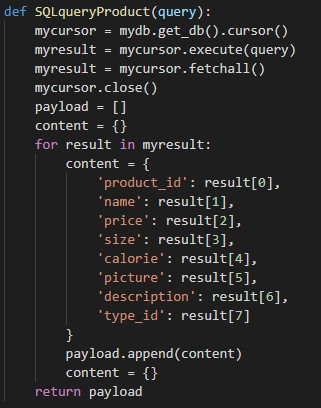
\includegraphics[width=0.5\textwidth]{drinks_1.jpg}
\end{center}
\caption{Funkcija, ki prebere podatke iz podatkovne baze}
\label{Drinks_DB_function}
\end{figure}

\begin{figure}[!htb]
\begin{center}
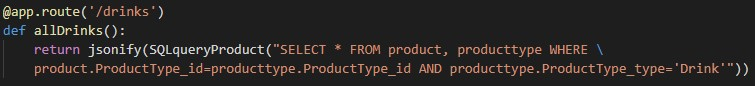
\includegraphics[width=14cm]{drinks_2.jpg}
\end{center}
\caption{Funkcija, ki na na relativno stran /drinks oglasi podatke}
\label{Drinks_URI}
\end{figure}

Tako smo dobili vmesnik, ki na zahtevo odjemalca odgovori s podatki v JSON formatu. Primer na sliki~\ref{ServerEX}, ko odjemalec zahteva podatke vseh pijač iz podatkovne baze (HTTP metoda GET). Strežnik omogoča tudi sprejemanje podatkov, vendar more biti zato ustrezna metoda HTTP. Metoda POST metodo smo uporabljali predvsem pri posredovanju podatkov strežniku, kateri so bili potrebni za zapis v podatkovno bazo. Spremljanje zahtevkov, ki prihajajo na strežnik, je mogoče preko vmesnika CLI, slika ~\ref{ServerEX2}, ki v primeru nepopolnosti prikaže ustrezno napako.

\begin{figure}[!htb]
\begin{center}
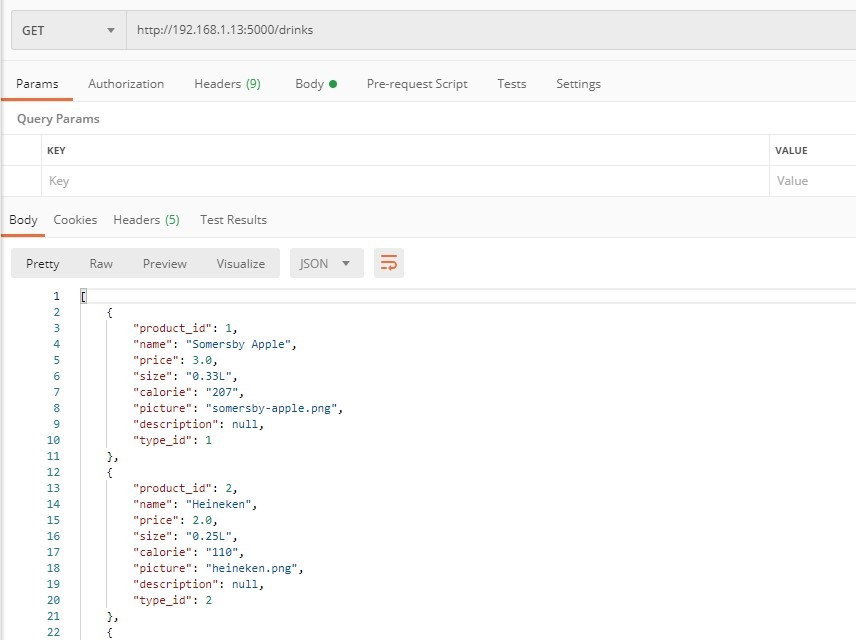
\includegraphics[width=10cm]{Server_example.jpg}
\end{center}
\caption{Primer serviranja podatkov na strežniku s programom Postman}
\label{ServerEX}
\end{figure}

\begin{figure}[!htb]
\begin{center}
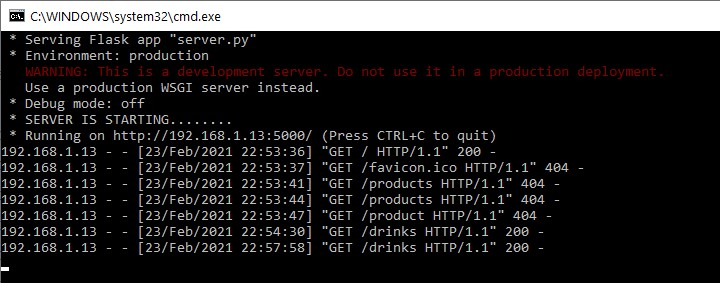
\includegraphics[width=12cm]{Server_example_2.jpg}
\end{center}
\caption{Primer spremljanja zahtevkov, ki prihajajo na strežnik}
\label{ServerEX2}
\end{figure}

Za potrebe pridobivanja podatkov v realnem času na strani odjemalca, smo potrebovali še spletni vtičnik SocketIO. Implementirali smo ga na strani strežnika in odjemalca, ki zagotavlja dvosmerno komunikacijo oziroma komunikacijo na podlagi dogodkov. Deluje na vseh platformah, brskalnikih ali napravah. Uporabili smo ga za obveščanje odjemalcov o spremembah v podatkovni bazi. Za to smo uporabljali funkcijo \sn{emit}, ki pomeni oddajanje. Omogoča dodajanje podatkov in izbiranje načina razpršenega oddajanja (ang. broadcast). To pomeni, da vsi prejemajo te informacije ob oddajanju na strani strežnika. Gre predvsem za splošne podatke, tako da ne more priti do zlorabe. Npr. ob spremembi naročila na strani gosta se le te razlike preverijo na strežniku in vpišejo v podatkovno bazo ter o tem obvesti natakarja s funkcijo \sn{emit}, ki vsebuje številko naročila v katerem je prišlo do sprememb. 


Poleg tega smo implementirali zaščito pred spreminanjem podatkov v podatkovni bazi. Ker aplikacija vsebuje nadzor nad določenimi podatki smo zato morali zagotoviti ustrezno varnost za urejanje le teh. Prvi nivo varnosti je avtorizacija odjemalca, kar pa seveda ni dovolj. Zahtevki za   


Poleg tega smo implementirali zaščito pred spreminanjem podatkov v podatkovni bazi. Ker aplikacija vsebuje nadzor nad določenimi podatki smo zato morali zagotoviti ustrezno varnost za urejanje le teh. Prvi nivo varnosti je avtorizacija odjemalca, kar pa seveda ni dovolj. Zahtevki za   


Poleg tega smo implementirali zaščito pred spreminanjem podatkov v podatkovni bazi. Ker aplikacija vsebuje nadzor nad določenimi podatki smo zato morali zagotoviti ustrezno varnost za urejanje le teh. Prvi nivo varnosti je avtorizacija odjemalca, kar pa seveda ni dovolj. Zahtevki za   

\begin{figure}[!htb]
\begin{center}
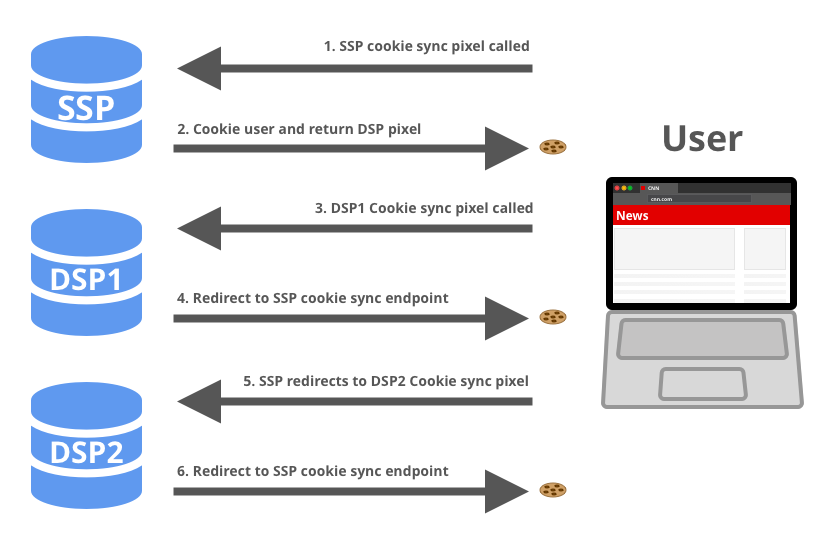
\includegraphics[width=14cm]{multi-partner-sync.png}
\end{center}
\caption{Funkcija, ki na na relativno stran /drinks oglasi podatke}
\label{Drinks_URI}
\end{figure}

\section{Odjemalec}

Odjemlaca bi načeloma lahko implementirali v spletnih tehnologijah (HTML, CSS, JS) ali pa v namenski mobilni aplikaciji. Mi smo se odločili za knjižnico in ogrodje Vue, ki je implementirano v programskem jezik JavaScript.  Naredili smo odziven in reaktiven vmesnik, ki deluje v realnem času. Vue je eden izmed mnogih kot npr. Angular, Ember, React,… poznan pa je predvsem zaradi enostavnosti za upravljanje in izvajanje testov. Vsem skupna reaktivnost, vendar v drugačnem pomenu besede. Reaktivnost \cite{reaktivnost}, je programska paradigma, ki nam omogoča, da se na deklarativni način prilagodimo spremembam. Tako deluje tudi reaktivnost v aplikacijah za razliko, da je podatek lahko vezan na več funkciji oziroma delov programske kode, ki se ob spremembi vrednosti posodobijo. Vue je namenjen izdelavi SPA projektov, saj vsebuje samo eno datoteko HTML. To prednost smo izkoristili s pomočjo ostalih knjižnic, ki so nam olajšale izdelavo aplikacije. Uporabili smo naslednje:
\begin{description}
\item[Vue CLI] velja kot standardno orodje za ekosistem Vue \cite{VueCLI}. Zagotavlja, da že pri gradnji novega projekta poveže različne dodatke med seboj. To omogoča razviljacu, da se bolj osredotoči na programiranje in ne na povezovanje njih v projekt. Zadeva izgleda nekako tako, da preko CLI vmesnika izbereš kakšen projekt želiš. Imaš seveda že privzete nastavitve, vendar omogoča tudi nastavljanje po meri. Sam sem uporabil Vuex, Vue-Router, ESLint in Vuetify.
\item[Vuex] je knjižnica za shranjevanje vrednosti v aplikacijah Vue.js \cite{Vuex}. Služi kot centralizirana baza podatkov za vse komponente v aplikaciji. 
\item[Vue-Router] je uradni usmerjevalnik za Vue.js \cite{VueRouter}. Integrira se globoko z jedrom Vue.js, tako da poenostavi izdelavo SPA aplikacij. Usmerjevalki je mišljen v smislu usmerjanja na druge komponente (angl. Component), ki v Vue.js predstavljajo druge poglede, lahko bi rekli podobno kot podstrani.
\item[ESLint] je orodje za prepoznavanje in poročanje o popravkih v programski kodi \cite{ESLint}. Cilj je narediti kodo bolj pregledno in urejeno, kar pripomore k izogibanju napak.
\item[Vuetify] je eden izmed mnogih uporabniških vmesnikov, ki je zgrajen na vrhu Vue.js \cite{Vuetify}. Za razliko od drugih vmesnikov je Vuetiy enostaven za učenje z več stotimi komponentami izdelanih po specifikacijah Material Design.
\item[Vue-devtools] je zgolj dodatek v brskalniku, ki omogoča lažje sledenje delovanja aplikacije in odpravljanju napak. 

\end{description}


Odjemalca smo razdelili v tri vloge oziroma dve aplikaciji. Ena aplikacija je namenjena natakarjem in kuharjem, ki se ločuje s prijavnim oknom in izgledom vmesnika. Druga aplikacija je namenjena samo gostom ter je sestavljena iz večih pogledov. Ločili smo jih zaradi varnosti, lažjega razvijanja in preglednosti, saj gre za dve popolnoma različni aplikaciji. Vse funkcionalnosti in delovanje ene in druge aplikacije je opisano v naslednjem poglavju. Sliki~\ref{Gost} in~\ref{NatakarGost} prikazujeti izgled obeh aplikacij.

\begin{figure}[!htb]
\begin{center}
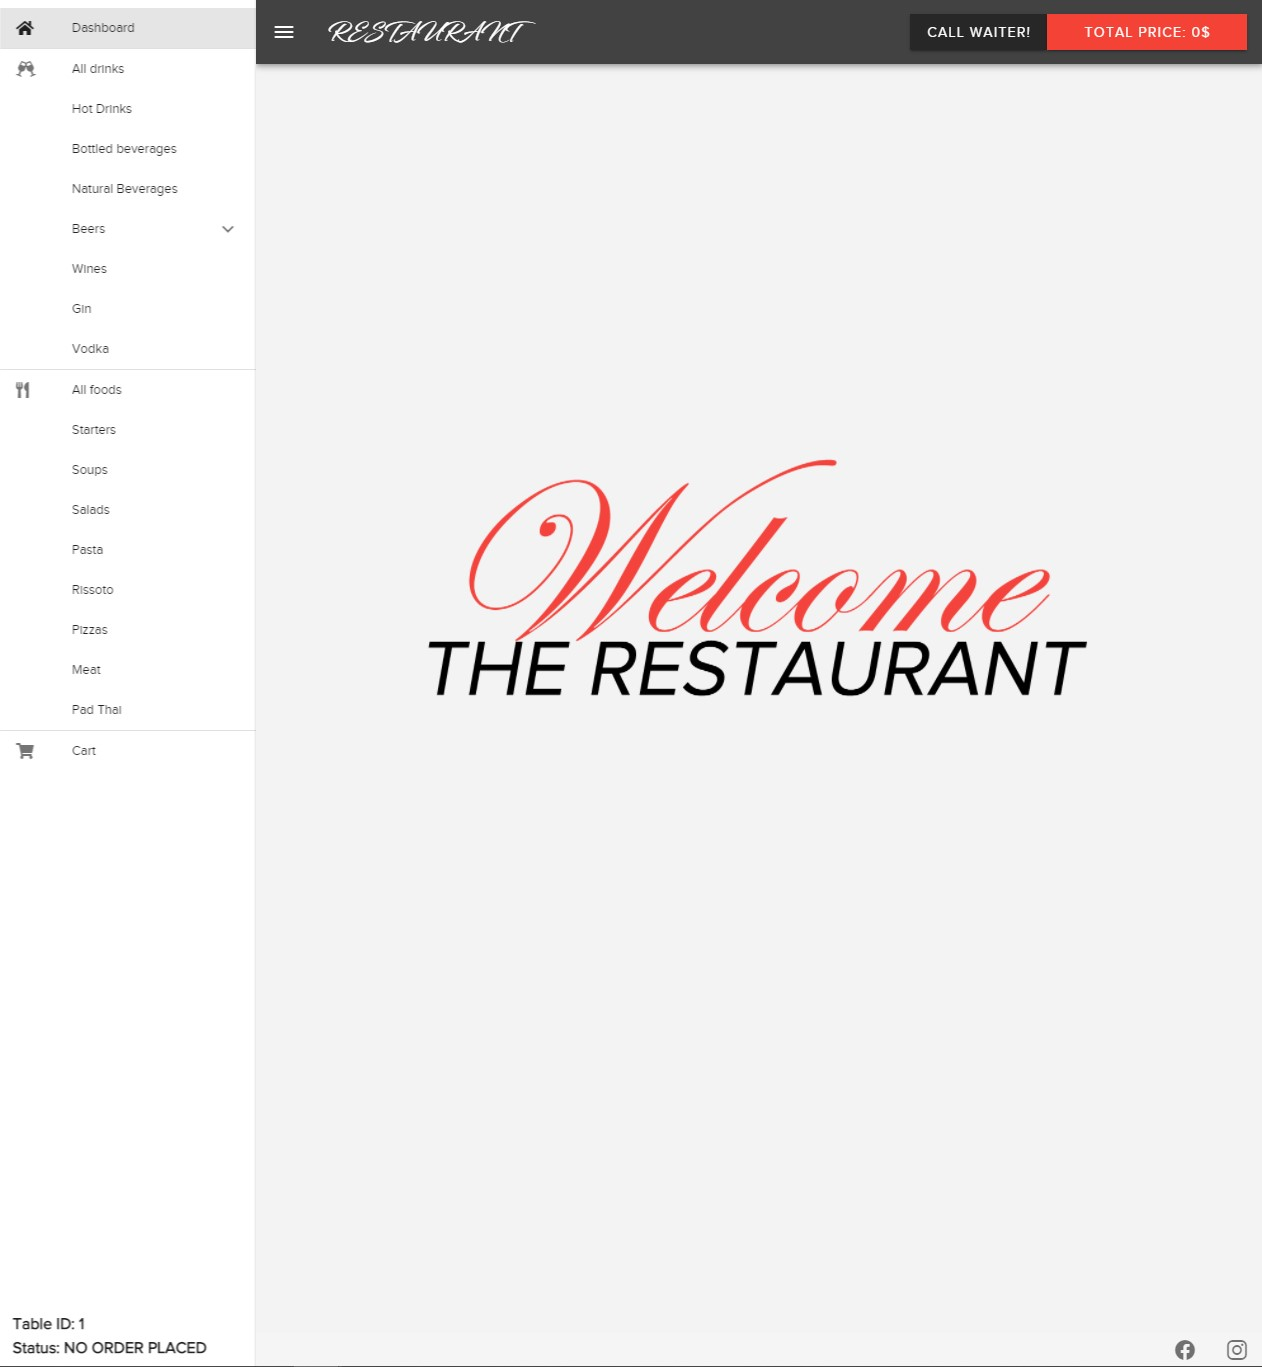
\includegraphics[width=12.5cm]{gost_1.jpg}
\end{center}
\caption{Spletni vmesnik za gosta}
\label{Gost}
\end{figure}

\begin{figure}[!htb]
\begin{center}
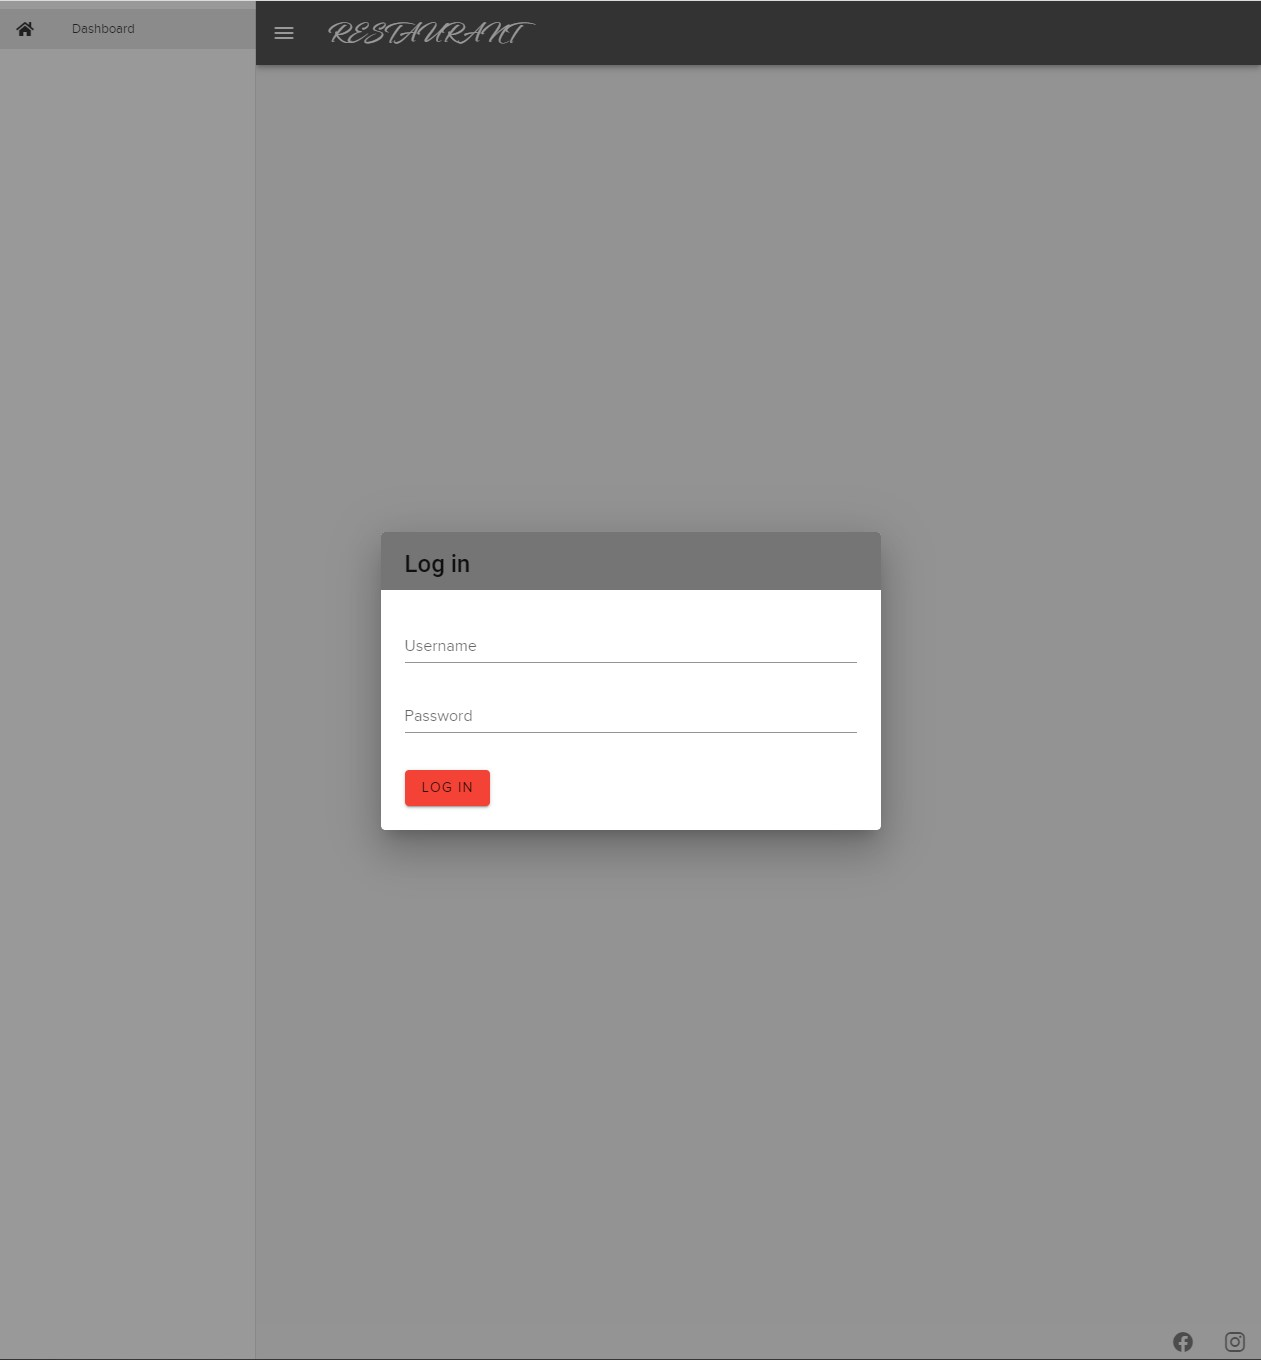
\includegraphics[width=12cm]{natakar-gost_1.jpg}
\end{center}
\caption{Spetni vmesnik za natakarja in kuharja}
\label{NatakarGost}
\end{figure}



Ena izmed pomembnih stvari pri obratovanje restavracije je čim hitrejša postrežba katero je mogoče izboljšati s čim hitrejšo komunikacijo. Zato smo, enako kot na strani strežnika, uporabili spletni vtičnik SocketIO. To smo vključili v obeh aplikacijah, in sicer za oddajanje naročil, posodabljanje naročil, obvečanju gosta o stanju naročila,... Najprej smo hoteli uporabiti samodejno osveževanje na določen časovni interval, vednar je uporaba spletnih vtičnikov precej bolj zanesljiva in točna. Slika~\ref{SocketIO_1} prikazuje seznam vseh vtičnikov, ki so uporabljeni na strani gosta.

\begin{figure}[!htb]
\begin{center}

\includegraphics[width=12cm]{socketio_1.jpg}
\end{center}
\caption{Spletni vtičniki v aplikaciji za gosta}
\label{SocketIO_1}
\end{figure}


Za pridobivanje podatkov na strani odjemalca smo uporabili Axios, ki je namenjen procesiranju zahtevkov  HTTP. To pomeni, da podatke, ki se oglašujejo na strani strežnika s pomočjo te knižnjice preberemo na strani odjemalca. 

\begin{figure}[!htb]
\begin{center}
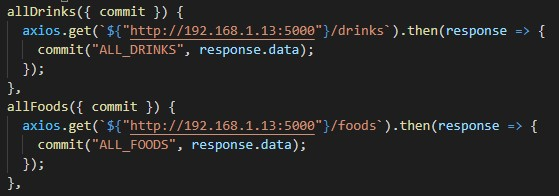
\includegraphics[width=12cm]{axios_1.jpg}
\end{center}
\caption{Način uporabe Axios v aplikaciji za gosta}
\label{axios_1}
\end{figure}


\chapter {Delovanje aplikacije}
\section{Vmesnik za gosta}
\section{Vmesnik za natakarja}
\section{Vmesnik za kuharja}

\chapter {Diskusija}

\chapter {Sklepne ugotovitve}
\newpage %dodaj po potrebi, da bo številka strani za Literaturo v Kazalu pravilna!
\ \\
\clearpage
\addcontentsline{toc}{chapter}{Literatura}
\bibliographystyle{plain}
\bibliography{literatura}


\end{document}

